\documentclass{beamer}
 
\usepackage{enumerate}
\usepackage{graphicx}
\usepackage[utf8]{inputenc}
\usepackage{lmodern}
 
%Information to be included in the title page:
\title{Dining Cryptographers Network}
\subtitle{An anonymous messaging system}
\author{Jack Wampler and Ian Martiny}
\institute{University of Colorado---Boulder}
\date{September 27, 2017}
 
 
 
\begin{document}
 
\frame{\titlepage}
 
\begin{frame}
\frametitle{Original Problem}
Three (or more) cryptographers are eating a meal at a restaurant. 
\vspace{0.5cm}

Afterwards the waiter announces that the meal has been paid for\pause
\vspace{0.5cm}

Only two options exist:
\begin{itemize}
    \item One of the diners secretly paid for the meal
    \item The NSA paid for the meal
\end{itemize}
\begin{figure}
    
\includegraphics[width=0.5\linewidth]{dining.jpg}
\end{figure}
\end{frame}

\begin{frame}{Original Problem (cont.)}
Each cryptographer respects the others' right to pay for dinner but need to know
if they did or the NSA paid
\begin{itemize}
    \item Essentially they need to send an anonymous 1 bit of information
\end{itemize}

First they need to get a shared bit between each pair (flip a coin behind a
menu)
\begin{figure}
    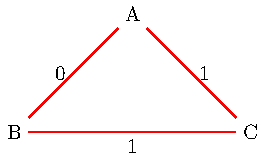
\includegraphics[width=0.5\linewidth]{DCTriangle.pdf}
\end{figure}
\end{frame}

\begin{frame}{Original Problem (cont.)}
\visible<1->{Each of the participants follows:}
\begin{itemize}
    \item \visible<1->{If they paid: announce the negation of the \texttt{xor} of
    things they know}
    \item \visible<2->{If they didn't pay: announce the \texttt{xor} of things
    they know}
    \item \visible<3->{\texttt{xor} announced data: 0 == NSA paid, 1 == someone
    paid}
\end{itemize}
\begin{figure}
    \visible<1->{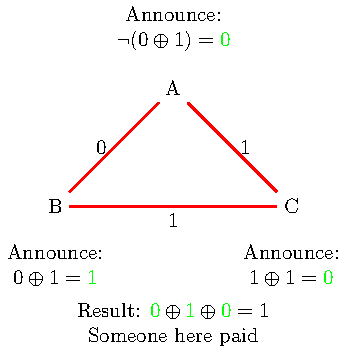
\includegraphics[width=0.4\linewidth]
    {DCTriangleApaid.pdf}}\hfill
    \visible<2->{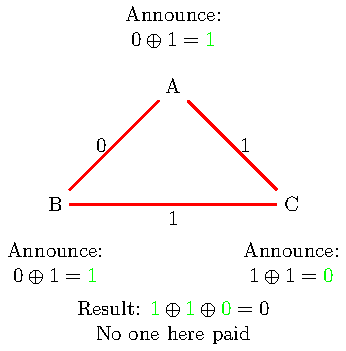
\includegraphics[width=0.4\linewidth]
    {DCTriangleNoPay.pdf}}
\end{figure}
\end{frame}

\begin{frame}{Dining Cryptographers Network}
This problem of sending one bit can be extended to sending multiple bits, i.e. a
message!

First issue, can't reuse bits! With repeated messages users gain information
about who is sending what.

\begin{figure}
    
\includegraphics[width=0.5\linewidth]{NotAnonymous.png}
\end{figure}
\end{frame}

\begin{frame}{DC Net methodology}
\begin{enumerate}[1.]
    \item Establish a shared secret between each pair 
    \begin{itemize}
        \item Diffie Hellman Key Exchange!
    \end{itemize}
    \item Use shared keys to seed separate PRNGs
    \begin{itemize}
        \item Lots of shared secrets! 
    \end{itemize}
    \item Same protocol as before!
\end{enumerate}

\begin{figure}
    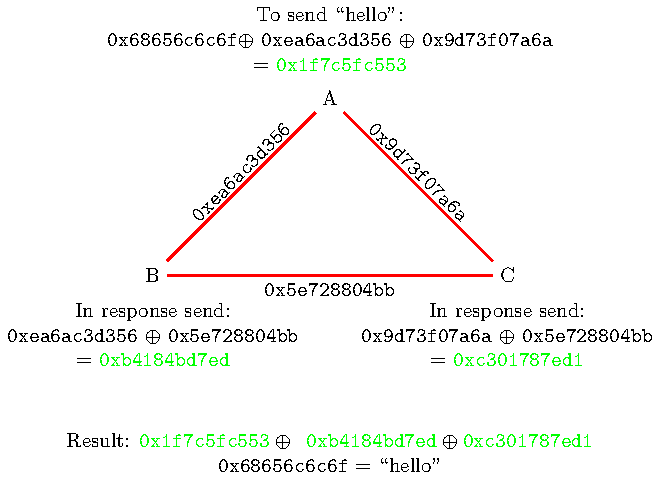
\includegraphics[width=0.6\linewidth]{DCTriangleMessage.pdf}
\end{figure}
\end{frame}

\begin{frame}{Design Considerations}
Our goal is to be anonymous
\begin{itemize}
    \item Clients can't just send out messages themselves
    \item Need a well-behaving server to handle broadcasting messages (playing
    role of waiter)
\end{itemize}

It appears there is no more negation in the previous example, but in fact
negation is simply the same as \texttt{xor}ing by 1. Thus our negate/not negate
idea is replaced with an \texttt{xor}
\end{frame}

\begin{frame}
\begin{center}
    \Large Demo
\end{center}
\end{frame}
\end{document}